\documentclass[11pt,a4paper]{scrartcl}

\usepackage[english]{babel}
\usepackage{standalone}
\usepackage{layouts}
\usepackage{geometry}
 \geometry{
 a4paper,
 margin=20mm
 }
%\usepackage{showframe}

%--Fonts---%
\newcommand\hmmax{0} %Avoid too many alphabets error
\newcommand\bmmax{0}
\renewcommand{\rmdefault}{ppl} % rm
\linespread{1.05}        % Palatino needs more leading
\usepackage[scaled]{helvet} % ss
\usepackage{courier} % tt
\usepackage{mathpazo} 
\usepackage{microtype}

%---Encoding---%
\usepackage[utf8]{inputenc}
\usepackage[T1]{fontenc}
\usepackage{lmodern}
\usepackage{csquotes}
\usepackage[ddmmyyyy,hhmmss]{datetime} %Compilation date

%---Math---%
\usepackage{amsmath,amsthm,amstext,amsbsy,amsfonts,amssymb,stackengine}
\usepackage{mathrsfs}
\usepackage{cancel}
\usepackage{bm}
\usepackage{mathtools}
\usepackage{mathdots}
\usepackage{thmtools}
\usepackage{array}
\usepackage{yhmath}
\usepackage{gensymb}
\usepackage{blkarray}
\usepackage{xfrac}

%---Plots---%
\usepackage{epstopdf}
\usepackage{gnuplottex}
\usepackage{calc}
\usepackage{graphicx}
\usepackage{color}
\usepackage{transparent}

%---Physics---%
\usepackage{physics}
\usepackage{siunitx}
\sisetup{
separate-uncertainty = true
}

%---Tables---%
\usepackage{booktabs}
\usepackage{multirow}

\setlength{\aboverulesep}{0pt} %removes annoying spaces in booktabs tables
\setlength{\belowrulesep}{0pt}
\setlength{\extrarowheight}{.75ex}
\setlength\parindent{0pt} 

%---Graphics & Plots---%
\usepackage{color}
\usepackage[usenames, dvipsnames, table]{xcolor} %colori
\usepackage{wrapfig}
\usepackage[font=footnotesize, labelfont=bf,
            labelformat=parens,
            labelsep=endash, justification=raggedright,
            singlelinecheck=on]{caption} %fancy captions
\usepackage{subcaption} 
\usepackage{pgf,tikz}
\usetikzlibrary{arrows}
\usetikzlibrary{tikzmark}
\usetikzlibrary{patterns}
\usepackage{soul}
\usepackage[framemethod=tikz]{mdframed}
\usepackage{fancybox}
\usepackage{framed}

%---Indeces, links, bibliography---%
\usepackage{imakeidx} %Indice analitico
\usepackage[stable]{footmisc}

%\usepackage{xr-hyper}
\PassOptionsToPackage{hyphens}{url}\usepackage{hyperref}  %hyperref va caricato sempre dopo footmisc, altrimenti le footnotes si buggano e riportano tutte alla prima pagina
%\usepackage[inline]{showlabels} %Draft

\usepackage[symbol=$\wedge$,numberlinked=false]{footnotebackref}
\makeindex[columns=2, title=Analytical index, options= -s indexstyle.ist]

\usepackage[backend=biber,sorting=none]{biblatex}
\renewbibmacro{in:}{}
\addbibresource{bibliography.bib}

%---Utilities---%
\usepackage{comment}
\usepackage{xspace}
\usepackage{marginnote}
\usepackage{ragged2e}
\usepackage{enumerate}
\usepackage{enumitem}
\usepackage{etoolbox}
\usepackage{xargs}                      % Use more than one optional parameter in a new commands
\usepackage{lipsum}  
\usepackage{float}

\usepackage{lipsum}  
\usepackage{float}
\usepackage{listings}
\usepackage[most]{tcolorbox}

\newcommand{\opx}[1]{\hat{\mathrm{#1}}}
\newcommand{\bb}[1]{\mathbb{#1}}

%%%%%%%%%% CODE LISTING %%%%%%%%%%%
%New colors 
\definecolor{codegreen}{rgb}{0,0.6,0}
\definecolor{codegray}{rgb}{0.5,0.5,0.5}
\definecolor{codepurple}{rgb}{0.58,0,0.82}
\definecolor{backcolour}{rgb}{0.95,0.95,0.92}
%Code listing style named "mystyle"
\lstdefinestyle{mystyle}{
  language=[90]Fortran,
  backgroundcolor=\color{backcolour},   commentstyle=\color{codegreen},
  keywordstyle=\color{magenta},
  numberstyle=\tiny\color{codegray},
  stringstyle=\color{codepurple},
  basicstyle=\ttfamily\footnotesize,
  breakatwhitespace=false,         
  breaklines=true,                 
  captionpos=b,                    
  keepspaces=true,                 
  numbers=left,                    
  numbersep=5pt,                  
  showspaces=false,                
  showstringspaces=false,
  showtabs=false,                  
  tabsize=2
}
%"mystyle" code listing set
\lstset{style=mystyle}

\usepackage{fancyhdr}
\pagestyle{fancy}
\fancyhf{} %Clear the previous header/footer

\lhead{Francesco Manzali}
\rhead{\today}
\lfoot{Neural Networks and Deep Learning A.A. 2020/21}
\rfoot{Assignment \exerciseNumber, page \thepage}

\newcommand{\exerciseNumber}{1}
\newcommand{\q}[1]{``#1''} 
\setlength{\parskip}{0cm}

\graphicspath{{Plots/}}
\begin{document}

%+Title
\title{Supervised Deep Learning}
\subtitle{Assignment \exerciseNumber}
\author{\large Francesco Manzali}
\date{\large \today}
\maketitle
\thispagestyle{fancy}
%-Title

%+Abstract
\begin{abstract}
  Two simple neural network models are developed for solving two supervised problems: function approximation (regression) and image recognition (multi-class classification). Generalization performance during training is evaluated through cross-validation, and improved by using an extensive random grid-search for hyperparameters, both regarding the learning process and the model's architecture.
\end{abstract}
%-Abstract


%Total length <= 6 pages, additional tables/figures can be added in a final appendix (optional)

\section*{Introduction}
Supervised Learning is a framework of machine learning in which a model learns \q{by example}, inferring useful patterns from a set of inputs (features) paired with their desired output (labels).

Formally, given a \textit{labelled dataset} $D = \{(\bm{x_i}, \bm{y_i})\}_{i=1, \dots, N}$, supervised learning trains a model $f\colon \bm{x} \to  \bm{y}$ such that $f(\bm{x_i}) \approx \bm{y_i} \> \forall i = 1, \dots, N$. This is done by iteratively minimizing a \textit{loss function}, which quantifies the difference (error) between predictions $f(\bm{x_i})$ and known labels $\bm{y_i}$. For neural networks, the minimization is achieved by the \textit{backpropagation} algorithm, along with an \textit{optimizer} such as Stochastic Gradient Descent. 

\medskip

In this assignment, two supervised learning tasks are examined:
\begin{enumerate}
    \item \textbf{Regression} (sec. \ref{sec:regression}): $100$ samples $(x,y)$ from an unknown scalar function $y=g(x)$ of one variable are given, and supervised learning is used to estimate the form of $g(x)$.
    \item \textbf{Classification} (sec. \ref{sec:classification}): $\num{60000}$ small ($28 \times 28$ pixels) labelled images of digits from the MNIST dataset \cite{MNIST} are used to build a classifier, effectively performing a limited optical character recognition.
\end{enumerate}

%Homework goals and the main implementation strategies chosen

\section{Regression \label{sec:regression}}
Learning a single smooth scalar function is usually an easy task. In this case, there are a few specifics of the dataset that make it more challenging:
\begin{itemize}
    \item Samples are few (only $100$)
    \item The training dataset is biased, in the sense that it does not cover uniformly the function's domain. In fact, two regions around $x = \pm 2$ are left out (fig.~\ref{fig:regression_results}, pag.~\pageref{fig:regression_results}).
\end{itemize}

\subsection{Methods}
Since the dataset is small and the problem is simple, overfitting is highly probable. Thus, it would be best to consider \q{small} neural networks, i.e. with \textit{few} hidden layers ($\leq 5$) and \textit{few} neurons per layer ($\leq 15$).

\medskip

The exact architecture, along with all the learning hyperparameters and the choice of the optimizer, is found by performing a random grid-search. To mitigate the dataset's small size, cross-validation with $k=5$ folds is used to estimate generalization performance. 

\medskip

The algorithm is as follows:
\begin{enumerate}
    \item A set of hyperparameters is sampled.
    \item The training dataset is divided in $k$ random subsets of equal size. One is put aside, and the whole training algorithm is run by using just the remaining $k-1$ sets as a labelled dataset. Then, generalization performance is evaluated on the set that was put aside. This procedure is repeated $k$ times, choosing a different set to put aside at each iteration. Finally, scores (e.g. the \textit{loss} values) are averaged over the $k$ repetitions.
\end{enumerate}

Hyperparameters are used also to choose the model's architecture. The network is always a sequence of fully-connected \textit{Linear} layers, with a non-linear activation in-between. The Mean Squared Error (MSE) is used as the loss function.

\medskip

Three \q{schemes} are devised for constructing the network:
\begin{itemize}
    \item \textit{same}: all layers have the same number of neurons (a random integer in $[2, 15]$). E.g. $(5, 5, 5)$ neurons for $3$ hidden layers.
    \item \textit{rise}: the first hidden layer has $2$ to $4$ neurons, and each subsequent layer has double the size of the previous one. E.g. $(3, 6, 12)$ neurons for $3$ hidden layers.
    \item \textit{rise-decrease}: same as \textit{rise}, but the \q{width} of layers increases up to the \q{middle} layer in the sequence, and then stays the same/decreases by half at each of the deeper layers. E.g. $(4, 8, 8, 4)$ neurons for $4$ hidden layers.
\end{itemize}
The same non-linear activation function, chosen randomly between \textit{ReLU} ($f(x) = \max(0, x)$), \textit{LeakyReLU} ($f(x) = \max(0,x) + 0.01 \min(0,x)$), \textit{Tanh} and \textit{Sigmoid} ($f(x) = [1+\exp(-x)]^{-1}$), is inserted after each hidden layer. No activation is needed for the output.

\medskip

The hyperparameters used for learning are the following:
\begin{itemize}
    \item \textbf{Optimizer}: random choice between SGD (with Nesterov momentum), Adam and RMSProp. The last two are more advanced, since they can \q{adapt} their learning rate automatically.  
    \item (Initial) \textbf{learning rate}: a random value $\lambda$ between $10^{-4}$ and $1$, chosen so that $\log \lambda$ follows a uniform distribution.
    \item \textbf{Batch size}: either $5$, $7$, $10$ or $15$.
\end{itemize}

Three types of regularization are considered, with at most one applied to any given network:
\begin{itemize}
    \item \textbf{Dropout}: a percentage $p$ of neurons from all layers (except the last) are randomly \q{switched off} during each forward pass of the training procedure, with $p$ between $10^{-4}$ and $10^{-1}$ (log-uniform). This reduces the \q{specialization} of neurons, distributing the computation and making the network more robust. During evaluation, all neurons are activated.
    \item \textbf{L1}: a term proportional to the sum of the absolute values of all weights is added to the loss function. This forces the weights to be smaller, and removes unimportant connections, making the network \q{sparser}. The proportionality factor is chosen between $10^{-5}$ and $10^{-1}$ (log-uniform).
    \item \textbf{L2}: a term proportional to the sum of weights squared is added to the loss function, forcing all weights to be much smaller. The proportionality factor is chosen between $10^{-5}$ and $10^{-1}$ (log-uniform).
\end{itemize}
In total, two random-grid searches ($500+$ trials) are executed: the first over all the search space, and the second over a smaller set of possibilities encompassing the best combinations found during the previous search.

%Model architectures and hyperparameters

\subsection{Results}
The final architecture consists of $3$ hidden layers with $(8, 16, 8)$ neurons each, a \textit{LeakyReLU} activation function, and the following hyperparameters for learning:
\begin{itemize}
    \item \textbf{Optimizer}: Adam, with $0.0083$ as initial learning rate
    \item No regularization
    \item Batch size of $7$
\end{itemize}
After $1000$ epochs of training (fig.~\ref{fig:learning_curves}), the final training MSE is $0.19 \pm 0.02$, while the validation MSE is $0.3 \pm 0.2$.

\medskip

Then, the model is re-trained over the whole $100$ samples of the training dataset for $1000$ epochs, and finally evaluated on a new \q{test} dataset, which was never used before. The results are plotted in fig.~\ref{fig:regression_results}. The performance is very good, with the test MSE ($\sim 0.1$) lying at the lower end of the MSE estimated during validation ($0.3 \pm 0.2$), probably due to the fact that the test dataset seems to be \q{less noisy} than the training one. Moreover, the two regions with no training samples, which contain two local maxima, are well-reconstructed. The estimation, however, is significantly lower than the ground-truth in these subsets, because it is biased to follow the neighboring (lower) points.

\medskip

The output of each neuron is shown in fig.~\ref{fig:regression_profiles}. Note how the complexity is higher the deeper is the layer. At the beginning, neurons can only differentiate low/high inputs, but already at the second layer they begin to specialize to model local maxima. In layer $3$ the output of several neurons already looks like the fitted function, while others do not activate at all. This opens the possibility of removing neurons, \q{pruning} the network, and reducing its computational cost while not affecting its performance. A histogram of all the weights of each layer is reported in the appendix (fig.~\ref{fig:weight_hist_regression}, pag.~\pageref{fig:weight_hist_regression}).
%Simulation results

\begin{figure}[H]
    \centering
    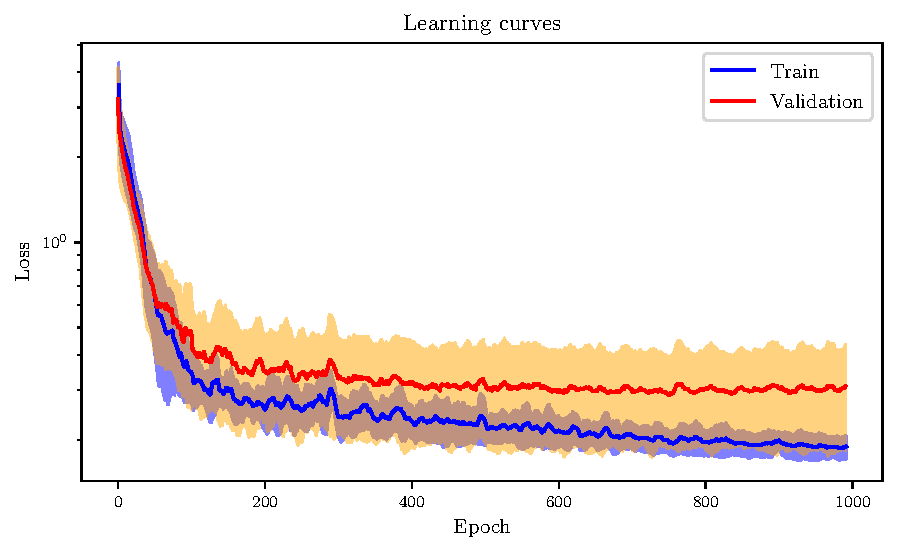
\includegraphics{../01_Regression/Plots/learning_curves.pdf}
    \caption{Learning curves for the regression task, with the best hyperparameters found by the random grid-search. Training and validation losses are averaged over a $5$-fold cross-validation, with the filled areas representing $\pm 1$ std variation. Note that the model converges around $400$ epochs, with the validation loss remaining stationary thereafter, and the training loss slightly decreasing (but remaining still within $\pm 1$ std of the validation one).\label{fig:learning_curves}}
\end{figure}
\begin{figure}[H]
    \centering
    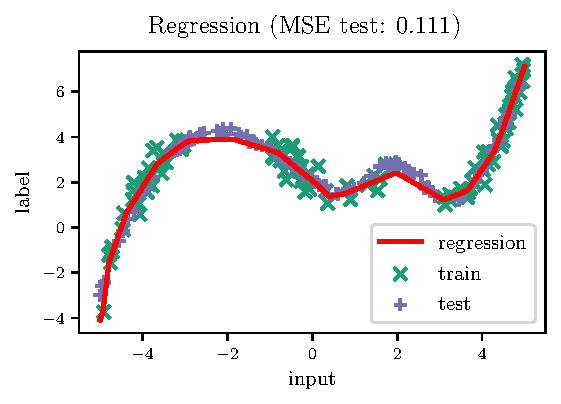
\includegraphics{../01_Regression/Plots/results.pdf}
    \caption{Final results for the regression task.\label{fig:regression_results}}
\end{figure}

\begin{figure}[H]
    \centering
    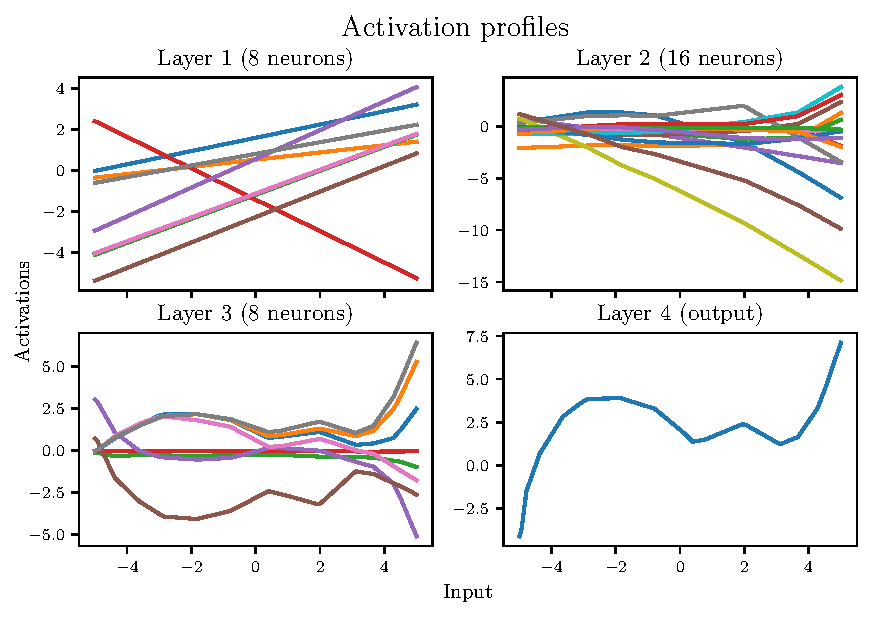
\includegraphics[width=0.8\textwidth]{../01_Regression/Plots/regression_profiles}
    \caption{Activation profiles for all layers in the network.\label{fig:regression_profiles}}
\end{figure}





\section{Classification \label{sec:classification}}

\subsection{Methods}
MNIST is a classic dataset for image recognition, consisting of \num{70000} images of digits of $28\times28$ pixels in size. Only a subset of it is used for training a multi-class classifier, while the rest is reserved for estimating the generalization performance. Specifically:
\begin{itemize}
    \item The first \num{60000} samples are used during training. $80\%$ of these (\num{48000}) are actually shown to the network to optimize its weights (\textit{training dataset}), while the remaining $20\%$ (\num{12000}) are used to estimate the performance during hyperparameter optimization (\textit{validation dataset}).
    \item The remaining \num{10000} samples form a \textit{test dataset} used only at the very end to estimate the generalization performance of the model.
\end{itemize}
The training dataset is \textit{augmented} by adding a random simple affine transformation to each batch during learning (random rotations of up to $\pm 10^\circ$, translations of up to $\pm 10\%$ and scaling of up to $\pm 10\%$). This means that, effectively, the model always sees different samples (dynamic data augmentation). Both the validation and test datasets are not affected in any way.

\medskip

The examined model is a Convolutional Neural Network with the fixed architecture shown in fig. \ref{fig:cnn_architecture}, chosen for its simplicity. 

\begin{figure}[H]
    \centering
    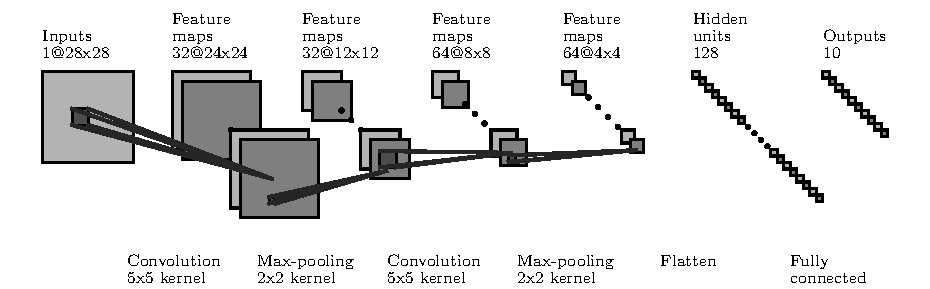
\includegraphics[width=\textwidth]{../02_Classification/Plots/convnet_fig}
    \caption{CNN Architecture. Image drawn with \href{https://github.com/gwding/draw_convnet}{gwding/draw\_convnet}.\label{fig:cnn_architecture}}
\end{figure}

A random grid search is used for choosing the hyperparameters for learning:
\begin{itemize}
    \item \textbf{Optimizer}: either Adam or SGD (with Nesterov momentum)
    \item \textbf{Learning rate}: a value in $[10^{-4}, 10^{-2}$ (log-uniform)
    \item \textbf{Batch size}: either $64$, $128$ or $256$
    \item \textbf{Activation function}: either \textit{ReLU} or \textit{LeakyReLU}.
    \item \textbf{Regularization}: either \textit{dropout} (in $[.05, .65]$, log-uniform, added after each hidden layer), \textit{L1} (in $[10^{-6}, 10^{-4}]$, log-uniform), \textit{L2} (in $[10^{-6}, 10^{-4}]$, log-uniform) or \textit{none}.
\end{itemize} 

\subsection{Results}
The best hyperparameters are found to be: Adam with $\lambda = \num{6e-4}$, ReLU activations, batch size of $64$ and no regularization. However, note that the grid-search evaluates each choice of hyperparameters over just $10$ epochs, to avoid taking too long. Since overfitting is not likely to happen immediately, the search suggests not to use regularization. But, at the end, one would like to train the model for longer, to maximize its performance. In that case, some amount of regularization must be considered. 

\medskip

Specifically, a small dropout value of $0.3$ is added, and the network is trained following all the other hyperparameters for $100$ epochs. Moreover, if the validation loss does not decrease for $10$ consecutive epochs, training is stopped prematurely. This idea, known as \q{early stopping}, helps to prevent overfitting. 

\medskip

After the final training, the model reaches $99.73\%$ of accuracy on the validation dataset, and $99.56\%$ on the test dataset. The learning curves are shown in the appendix (fig.~\ref{fig:learning_curve_cnn}, pag.~\pageref{fig:learning_curve_cnn}), along with the histograms of the weights (fig.~\ref{fig:weight_hist_cnn}), the confusion matrix (fig.~\ref{fig:confusion}) and some examples of misclassifications (fig.~\ref{fig:misclassified}).

\medskip

To see what the network is doing, it is useful to plot some filters. For instance, fig.~\ref{fig:cnn_weights} shows the kernels of the first convolutional layer. These appear to be mostly edge detectors: filter $24$ detects horizontal lines, filter $15$ oblique ones, and filter $17$ vertical ones. Their effect is more apparent when they are applied to a sample, as shown in fig.~\ref{fig:cnn_features}. 


\begin{figure}[ht]
    \centering
    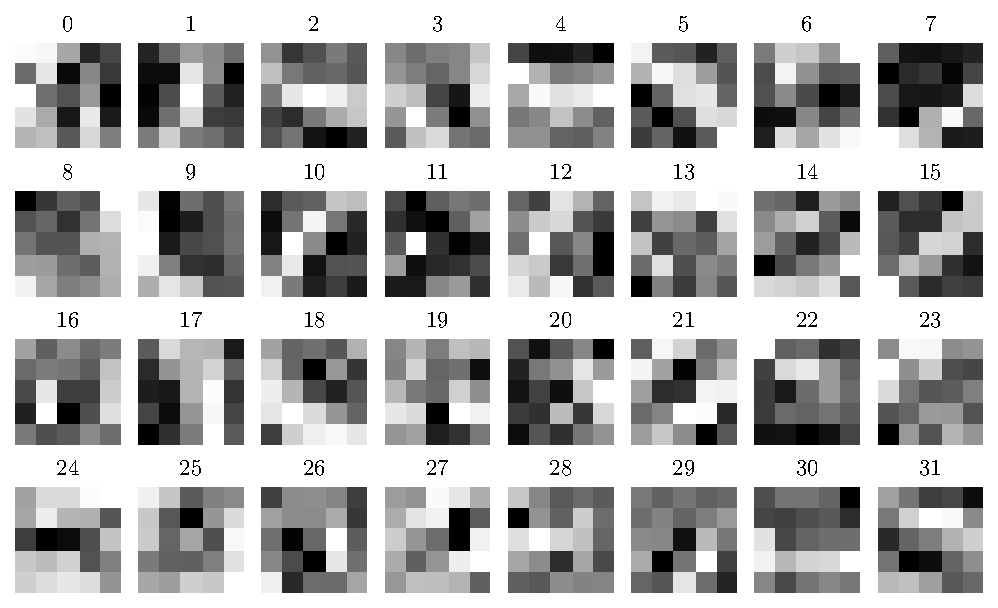
\includegraphics[width=0.8\textwidth]{../02_Classification/Plots/cnn_weights}
    \caption{Plot of the weights from the filters in the first convolutional layer.\label{fig:cnn_weights}}
\end{figure}

\begin{figure}[ht]
    \centering
    \begin{subfigure}[c]{0.3\textwidth}
        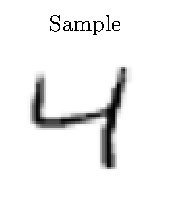
\includegraphics[width=\textwidth]{../02_Classification/Plots/feature_maps_cnn_sample}
    \end{subfigure}%
    \begin{subfigure}[c]{0.7\textwidth}
        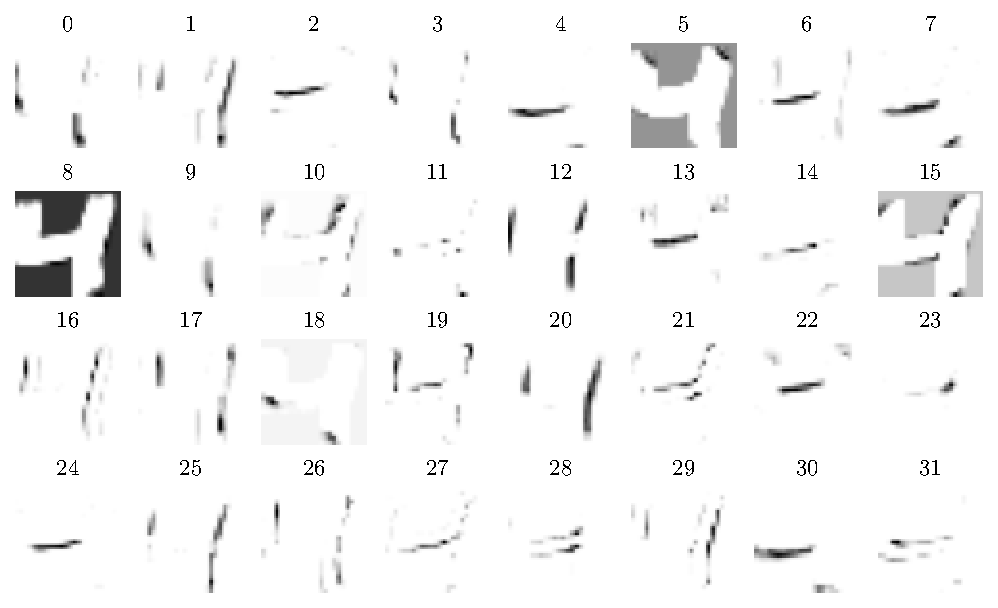
\includegraphics[width=\textwidth]{../02_Classification/Plots/feature_maps_cnn}
    \end{subfigure}
    \caption{Feature maps $0-31$ obtained by applying the filters from fig.~\ref{fig:cnn_weights} to the sample shown to the left. \label{fig:cnn_features}}
\end{figure}



%\the\textwidth
\printbibliography

\clearpage

\section*{Appendix}
This section contains some additional figures, showing a few more glimpses on the performance of the models and their inner workings.

\begin{figure}[htp]
    \centering
    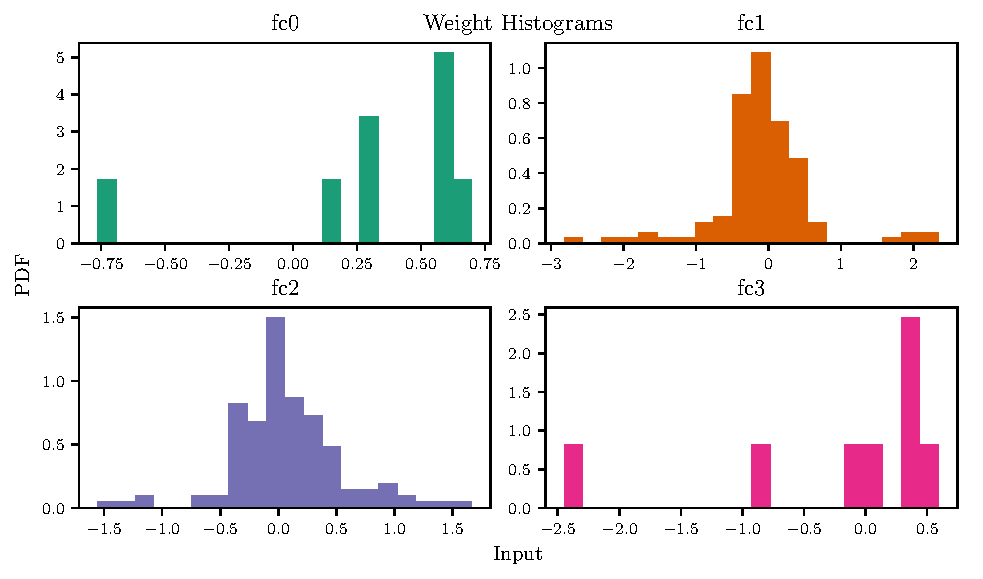
\includegraphics[width=0.88\textwidth]{../01_Regression/Plots/regression_weight_hist}
    \caption{Histograms of weights for the neural network used in the regression task.\label{fig:weight_hist_regression}}
\end{figure}

\begin{figure}[htp]
    \centering
    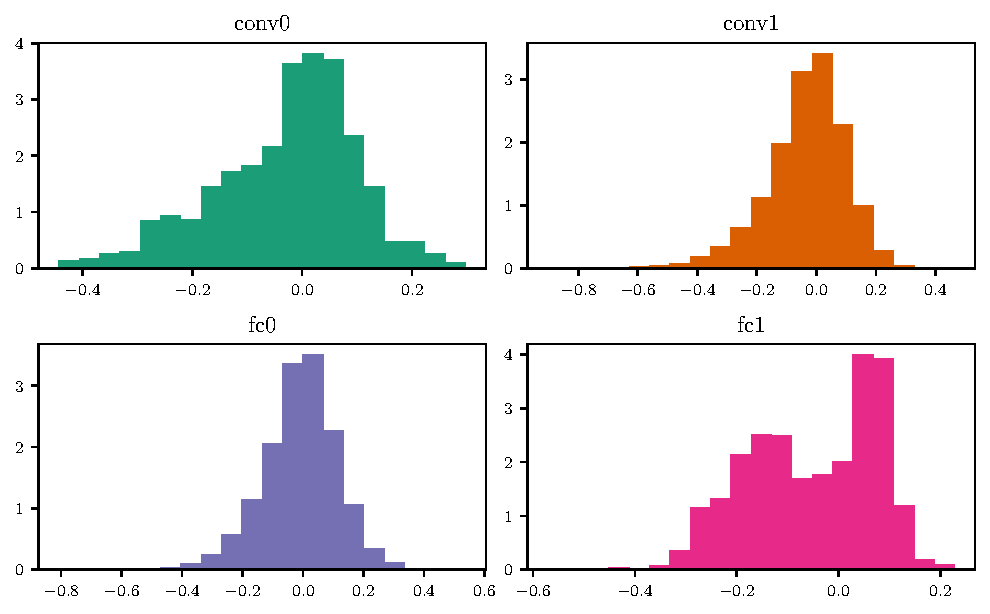
\includegraphics[width=0.8\textwidth]{../02_Classification/Plots/weight_histogram}
    \caption{Histogram of weights for the neural network used in the classification task.\label{fig:weight_hist_cnn}}
\end{figure}

\begin{figure}[htp]
    \centering
    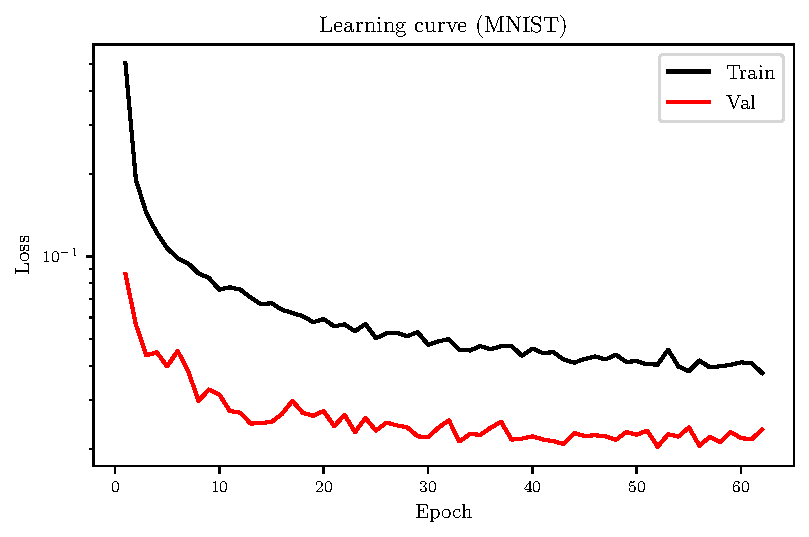
\includegraphics[width=0.7\textwidth]{../02_Classification/Plots/learning_curves_cnn}
    \caption{Learning curve for the final training of the MNIST classifier. Note that the validation curve is significantly lower than the training one. This is because the model uses dropout for regularization, which is active just for the training part. Moreover, training samples are always different at each epoch, due to the random transformations of the augmentation procedure, while the validation dataset is always the same. \label{fig:learning_curve_cnn}}
\end{figure}


\begin{figure}[htp]
    \centering
    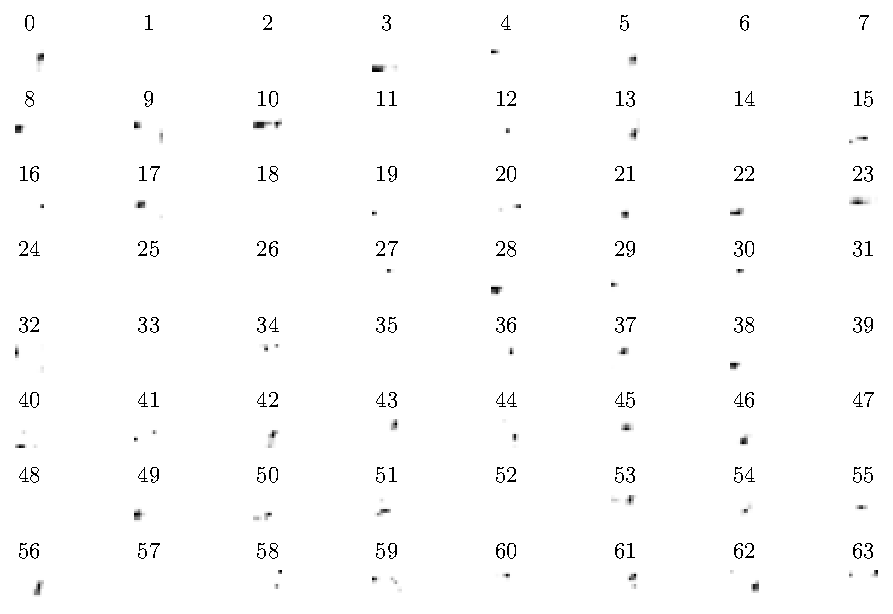
\includegraphics[width=0.9\textwidth]{../02_Classification/Plots/feature_maps_cnn_conv2}
    \caption{Feature maps of the second convolutional layer of the CNN used for the classification task, with the same sample from fig.~\ref{fig:cnn_features}. Since this layer is preceded by a maxpool operation, the maps are much smaller. \label{fig:cnn_features2}}
\end{figure}

\begin{figure}[htp]
    \centering
    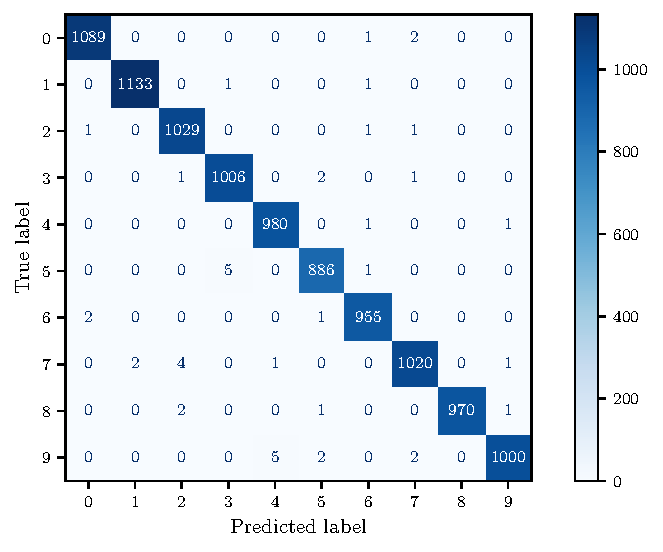
\includegraphics[width=0.8\textwidth]{../02_Classification/Plots/confusion_matrix}
    \caption{Confusion matrix for the MNIST classifier.\label{fig:confusion}}
\end{figure} %TODO colorbar not working -> Works when compiled by VSC, not by Bakoma

\begin{figure}[htp]
    \centering
    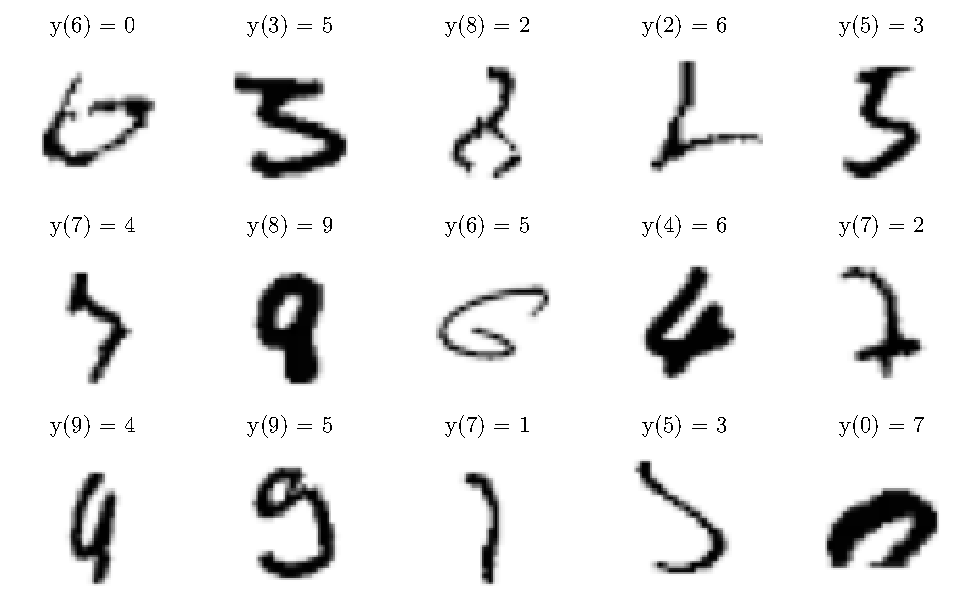
\includegraphics[width=0.8\textwidth]{../02_Classification/Plots/misclassified.pdf}
    \caption{Some of the samples from the test dataset that are misclassified by the CNN model, labelled as $y(\mathrm{true\_label})=\mathrm{wrong\_predicted\_label}$.\label{fig:misclassified}}
\end{figure}



\end{document}
